% !TEX root = thesis.tex

\chapter*{Preface}
% \addcontentsline{toc}{chapter}{Preface}

We usually associate the three usual dimensions with length, width and height, as well as a fourth dimension with time. 
However, mathematically, dimensions are essentially a construct and do not have a fixed meaning.
By associating each dimension with a variable, they can be used to represent any kind of characteristic that is \emph{parametrisable}.
Within this thesis, higher-dimensional geometric representations are thus used to model various aspects of geographic information, such as the typical geographic coordinates, but also time and scale.

At the end of the 19th century, a couple of non-scientific books were notable for popularising thinking about dimensions, the satyrical \emph{Flatland: A Romance of Many Dimensions} \citep{Abbott84} (\reffig{fig:flatland}), and the more serious \emph{A New Era of Thought} \citep{Hinton88}.
These books used analogies between familiar 0D--3D situations and those in higher dimensions, attempting to give readers an intuitive feeling of what these abstract higher dimensions are like.
Plenty of others have continued to follow in their footsteps, including some in popular media (\reffig{fig:futurama}).

\marginpar{
\captionsetup{type=figure}
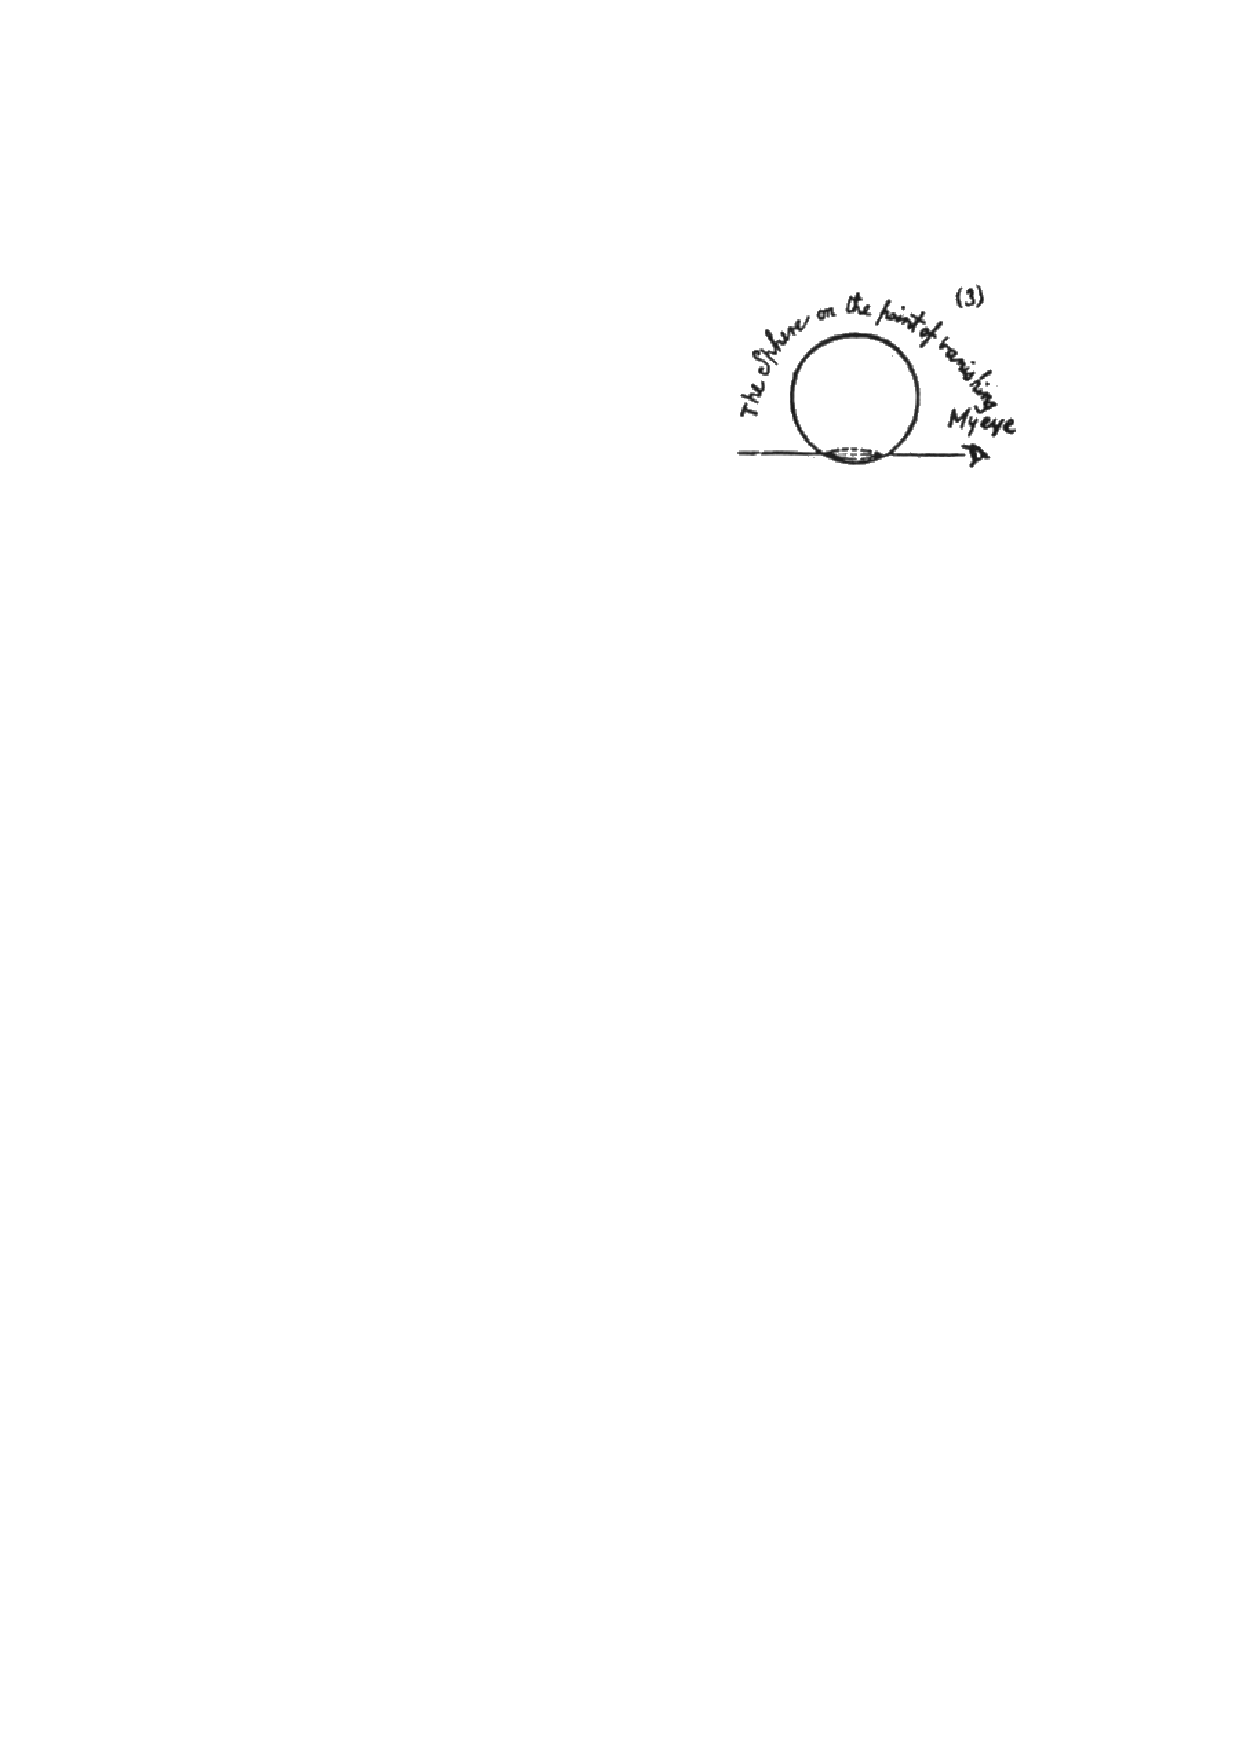
\includegraphics[width=\marginparwidth]{figs/flatland}
\caption[Sphere tries to explain the nature of 3D space to Square]{As Sphere tries to explain the nature of 3D space to Square by passing through its plane of view: `\emph{You cannot indeed see more than one of my sections, or Circles, at a time; for you have no power to raise your eye out of the plane of Flatland; but you can at least see that, as I rise in Space, so my sections become smaller}' \citep{Abbott84}.}
\label{fig:flatland}
}

\marginpar{
\captionsetup{type=figure}
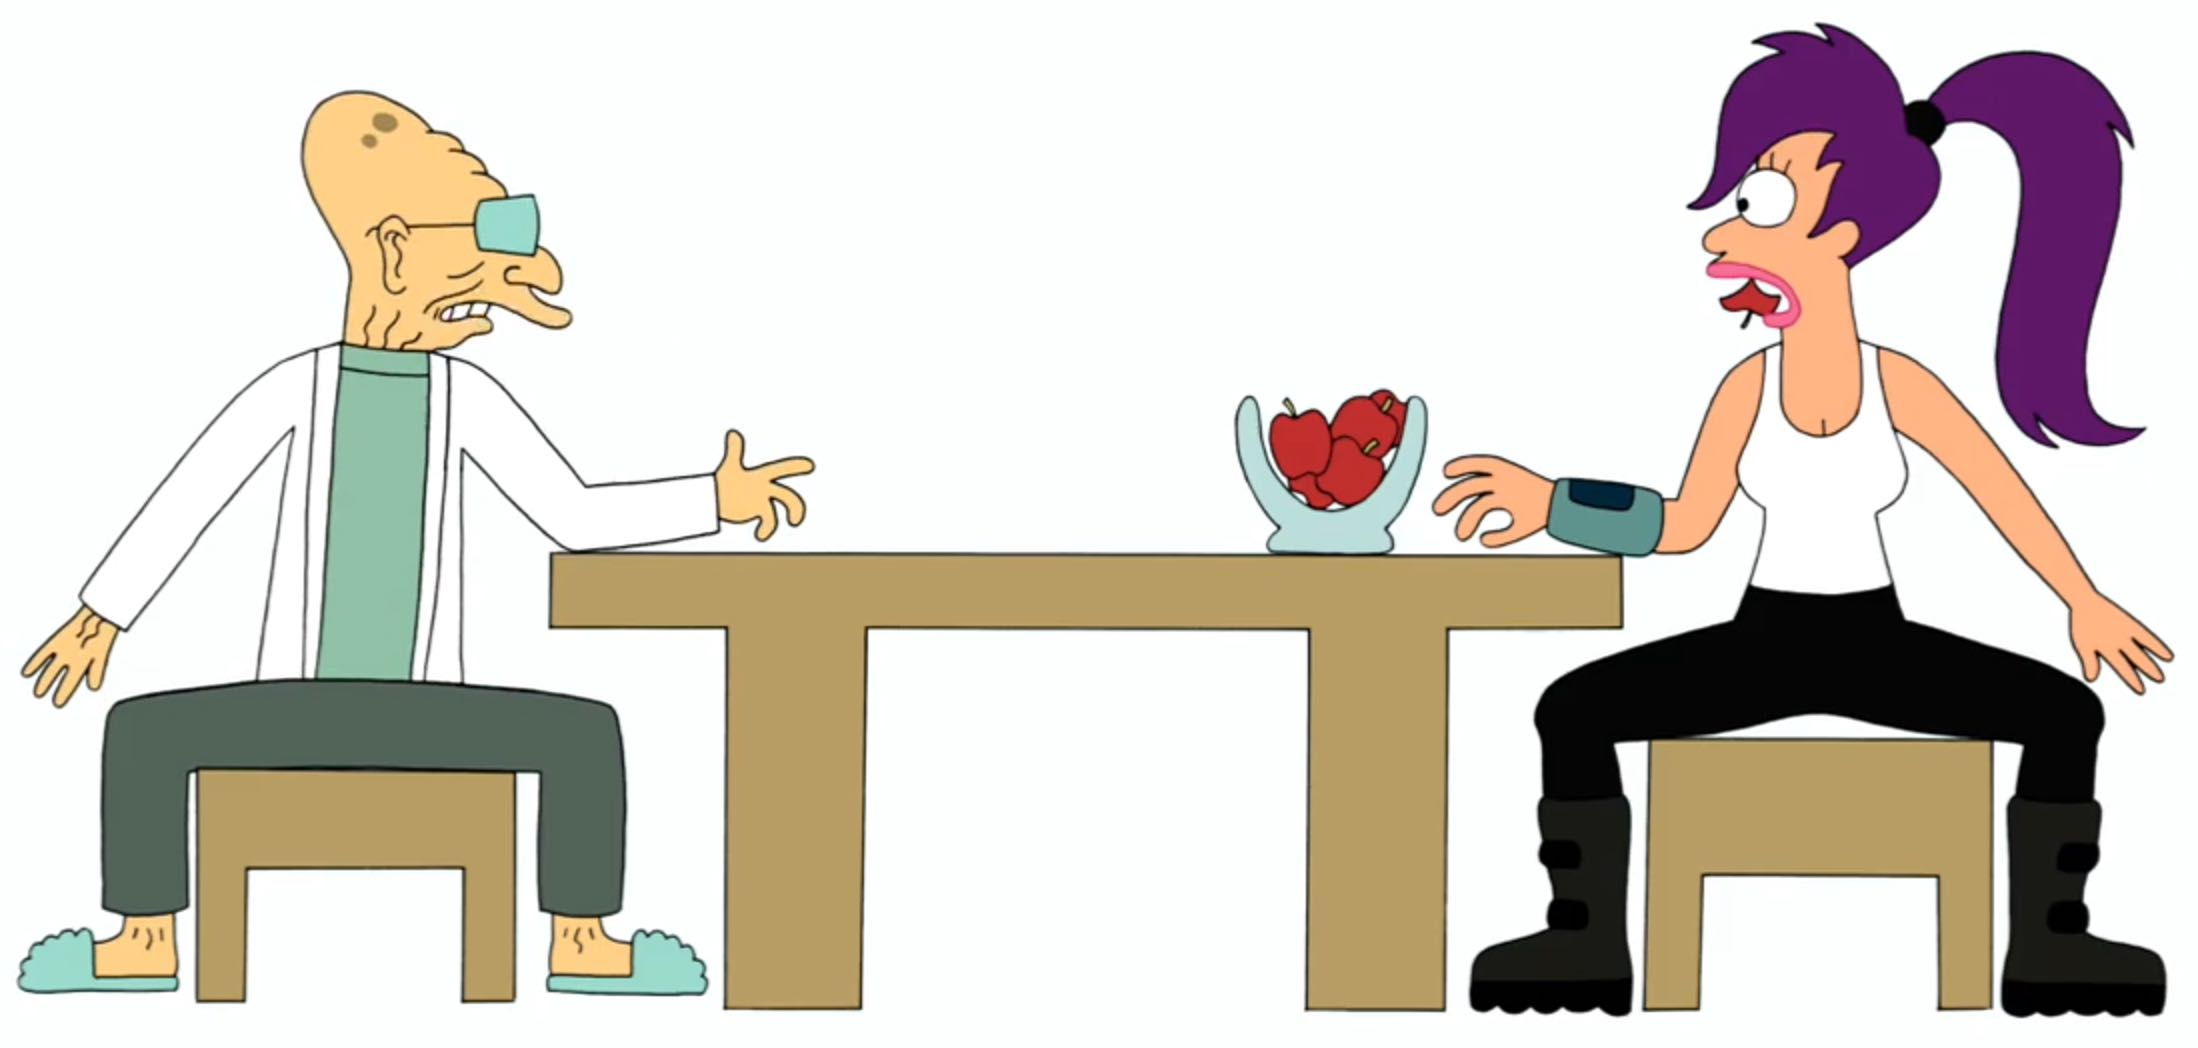
\includegraphics[width=\marginparwidth]{figs/futurama}
\caption[Farnsworth explains why a two-ended digestive system cannot exist in 2D]{As Professor Farnsworth explains why a two-ended digestive system cannot exist in a 2D world: `\emph{As you can see, or rather can't see, but take my word for it, such a digestive system would divide a 2D being into separate pieces.}'. From Futurama season 7 episode 14.}
\label{fig:futurama}
}

This thesis uses formal descriptions for data structures and algorithms, but also similar intuitive explanations and analogies across different dimensions, offering explanations of higher-dimensional problems based on our intuitive knowledge of similar 2D and 3D cases.
I hope that the result is approachable and serves to broach the subject in a practical way, using real-world data, implementing ideas into software prototypes and explaining concepts through practical examples.

\section*{About this thesis}

During the past 4+ years I have found many things to love about the scientific process, but many things to hate about how its results are released and published.
More than a century after Leo Tolstoy's \emph{Letter to the Free Age Press}\footnote{\url{https://en.wikisource.org/wiki/Letter_to_the_Free_Age_Press}} and 20 years after Stevan Harnad's \emph{subversive proposal}\footnote{\url{https://en.wikipedia.org/wiki/Subversive_Proposal}}, it is rather sad to see that so much science is still kept behind paywalls or stymied by legal restrictions even when it is taxpayer-funded.
% \footnote{Something that is true for much industry research as well, which is paid from tax exemptions on R\&D}.
This is not only damaging to scientific discourse, but it keeps important knowledge from the public at large, including educators and legislators.
% The industry is of course all too glad to fill this void with duplicitous studies, which are often pushed by lobbyists in slick packaging.

At the same tim, there is a concerted effort to restrict knowledge creation and creative expression through draconian intellectual property laws, including providing IP holders with special (extra)legal privileges and misappropriating author and user rights while extending already excessive copyright terms.
Plenty of laws have been enacted on the matter with a complete lack of transparency, despite obvious harm to users and evidence to a lack of economic benefits \citep{Hargreaves11,Reda14,EFI15}.
% For all intents and purposes, a system ostensibly created for the protection of authors have been co-opted by the copyright industries.

By releasing this thesis' contents into the public domain and making its source publicly available, I wish to make a small statement about how I would like science to be distributed in the future---openly and without restrictions.
Open access journals are a step in the right direction\footnote{Even as some of them have abusive fees that bear no relation with the marginal cost of internet distribution.}, but I hope it is not too long before we are able to get rid of journals and publishers altogether.

Following in the same spirit, the source code of the main prototype implementations that were developed during this PhD project have also been made publicly available under permissive licences, which are linked to in the corresponding parts of this thesis.
% , even if the code quality is closer to a proof sometimes lower than I would like.
As others have pointed out before me, there is a great disparity between the alleged importance of scientific evidence and widespread acceptance of not disclosing software implementations \citep{Morin12,Joppa13}.
More cogently, \emph{there is no such thing as reproducibility without source code} \citep{Ince12}.

\section*{Acknowledgements}

My utmost thanks go to my supervisors, \textbf{Hugo} and \textbf{Jantien}.
They not only provided me with the opportunity to work on this PhD, but were always there with good ideas, and all the guidance and support anyone could wish.

I am very much grateful to everyone else in the \textbf{3D geoinformation} group in my time there (\textbf{Filip}, \textbf{Liu}, \textbf{Ravi}, \textbf{Sisi} and \textbf{Zhiyong}).
I feel privileged to have been a part of it from the start and to have been able to contribute to it with my grain of sand.

I am also thankful to everyone at \textbf{GIS Technology} (\textbf{Edward}, \textbf{Elfriede}, \textbf{Marian}, \textbf{Martijn}, \textbf{Radan}, \textbf{Theo}, \textbf{Tjeu}, \textbf{Peter} and \textbf{Wilko}), where I started this PhD.
Special thanks go to \textbf{Guillaume} for hosting me in Lyon and helping me with his CGAL packages.

Last but not least, I thank my mother, \textbf{Kimiyo}, who has always been there supporting me, and to my friends in Mexico, the Netherlands and elsewhere, who made sure I always had things to enjoy outside work.

Thank you all.